\chapter*{Introducción}
 
El libro de Claude Shannon \textit{Mathematical Theory of Cryptography} (1945) y su ampliación posterior, \textit{Mathematical Theory of Communication} (1948) dieron a luz a dos disciplinas hoy plenamente establecidas, la teoría de información y la teoría de códigos.

El objetivo principal de la teoría de códigos y de la teoría de la información es el de establecer mecanismos de comunicación que sean eficientes y fiables en ambientes posiblemente hostiles.
La eficiencia requiere que la transmisión de la información no necesite de demasiados recursos, sean materiales o temporales.
Por otro lado, la fiabilidad requiere que el mensaje recibido en una comunicación sea lo más parecido posible, dentro de unos márgenes de tolerancia, al mensaje original.

La teoría de la información se encarga del estudio tanto de la representación de la información como de la capacidad que tienen los sistemas para transmitir y procesar la información. 
Por otra parte, la teoría de códigos se basa en los resultados de la teoría de la información para el el diseño y desarrollo de modelos de transmisión de información mediante herramientas algebraicas.

\begin{figure}
  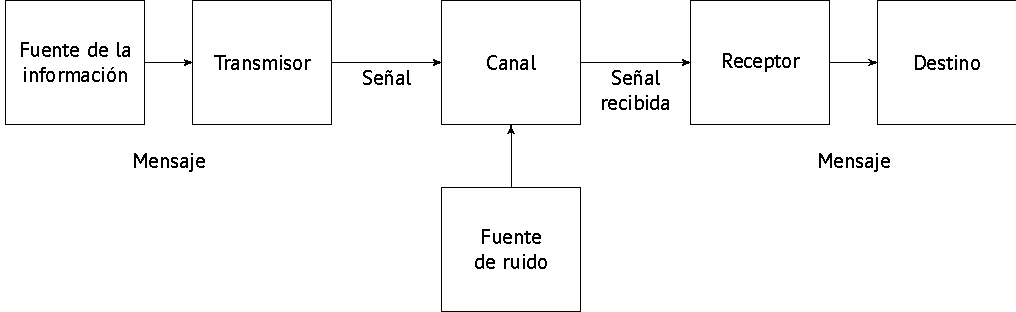
\includegraphics[width=\textwidth]{assets/shannon-communication-model.pdf}
  \caption*{Modelo de comunicación de Shannon}
\end{figure}

El filósofo inglés Francis Bacon ya afirmó en el año 1623 que únicamente son necesarios dos símbolos para codificar toda la comunicación.

\blockquote[{\cite[30]{dyson_catedral_2015}}]{La transposición de dos letras en cinco emplazamientos bastará para dar 32 diferencias [y] por este arte se abre un camino por el que un hombre puede expresar y señalar las intenciones de su mente, a un lugar situado a cualquier distancia, mediante objetos ... capaces solo de una doble diferencia.}
